\chapter{分子发光分析}

\begin{introduction}
	\item 三种分子发光产生的原理(理解)
	\item 荧光定量分析有关概念
	\item 荧光分光光度计(熟悉)
\end{introduction}


%设计方案:
%1.定义、概念、原理,做个环境
%2.公式、符号说明环境
%3.步骤、结构、小点:列表
%4.对比:表格

\section{分子发光产生的原理}

\begin{emptytcb*}{荧光的原理}{}
	受光激发的分子从第一激发单重态的最低振动能级回到基态所发出的辐射。寿命为10-8~ 10-11s。由于是相同多重态之间的跃迁,几率较大,速度快,速率常数$k_f$为$106~109 s-1$。
\end{emptytcb*}

\begin{emptytcb*}{磷光的原理}{}
	是由第一激发单重态的最低能层,经系间跨越跃迁到第一激发三重态,并经振动弛豫至最低振动能层,然后跃迁回到基态发生的。由于磷光的产生伴随自旋多重态的改变,辐射速度远小于荧光,磷光寿命 为10-4~10 s。
\end{emptytcb*}

\begin{emptytcb*}{化学发光的原理}{}
	 某些物质在进行化学反应时,由于吸收了反应时产生的化学能,而使反应产物分子激发至激发态,受激分子由激发态回到基态时,便发出一定波长的光。这种吸收化学能使分子发光的过程称为化学发光。化学发光也发生于生命体系, 这种发光称为生物发光。
\end{emptytcb*}

\begin{figure}
	\centering
	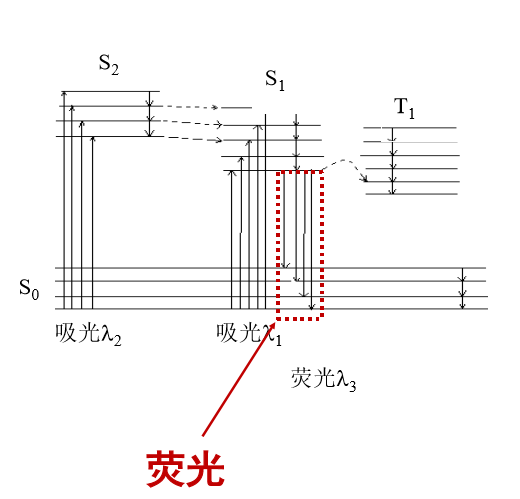
\includegraphics[width=0.7\linewidth]{chp4_flu_principle}
	\label{fig:chp4fluprinciple}
	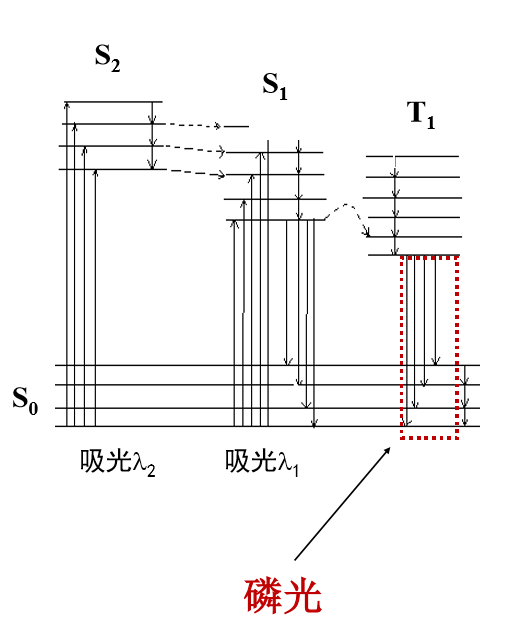
\includegraphics[width=0.7\linewidth]{chp4_phos_principle}
	\label{fig:chp4phosprinciple}
	\caption{}
\end{figure}



2、什么是荧光量子产率?和物质结构的关系?荧光的定量分析的基础(公式)?什么是荧光猝灭?
荧光量子产率(Φ):
\begin{definition*}{荧光量子产率}{}
	 表示物质发射荧光的能力,如果一个分子将吸收的光子全部释放,则其量子产率为$100\%$。
\end{definition*}

Φ与失活过程的速率常数k有关:

凡是使荧光速率常数kf增大而使其他失活过程(系间窜越、 外转换、内转换)的速率常数减小的因素都可使荧光增强。
荧光与分子结构的关系:
A.跃迁类型:π*→π的荧光效率高,系间跨越过程的速率常数小,有利于荧光的产生,故发射 π*→π跃迁比π*→n跃迁更常见;
B.共轭效应:提高共轭度有利于增加荧光效率并产生红移;
(1)芳香族化合物的荧光最常见且最强,大多数未取代芳烃在溶液中发荧光,随着环的数目和共轭度增加,荧光峰红移,Φ↑。简单杂环化合物不发荧光,但具有稠环结构的杂环化合物都发荧光;
(2)任何有利于提高π-电子共轭度的结构改变,都将提高荧光量子产率,或使荧光波长向长波长方向移动;
(3)电子共轭程度越大,越容易产生荧光;环越大,发光峰红移程度越大,发光往往越强;
(4)共轭环数相同的芳香族化合物,线性环结构的荧 光波长比非线性者要长。
C. 刚性平面结构:
可降低分子振动,减少与溶剂的相互作用,故具有很强的荧光;
D. 取代基效应:
(a)芳环上有羧基、羰基、亚硝基、巯基等吸电 子基团取代时,荧光减弱;
取代基的n电子云并不与芳环上π电子云共平面;
(b)给电子取代基如-OH、-NH2、-CN、-OCH3等会使荧光强度增加;
取代基上的n电子的电子云几乎和芳环上的π轨道平行, 因而共享了共轭π电子结构,产生了p- π共轭效应,扩大了共轭双键体系。
(c)重原子效应: 含有重原子的分子中,使系间窜跃的几率大,荧光强度随 卤素相对原子质量的增强而减弱,磷光增强。如:Br,I;
(d)取代基的位置:
(1)对位、邻位取代增强荧光,间位取代抑制荧光;
(2)双取代或多取代基的影响较难预测;
(3)取代基之间能形成氢键增加分子的平面性,荧光增强;
(4)两种性质和作用不同的取代基共存时,其中一个起主导作用。
荧光的定量分析的基础:
荧光物质浓度很稀时,所发射的荧光相对强度If可用下式表示:

随着荧光物质浓度增加,吸光度A增加,相对荧光强度增加。
(a)当溶液很稀,吸光度A<0.05时,e-A≈1-A,则 

在一定条件下,用𝐼0一定的入射光激发荧光溶液时,其发射的荧光强度与荧光物质的浓度成正比。
(b)当溶液的A≥0.05时将产生浓度效应,使荧光强度与浓度的关系偏离线性。

荧光猝灭:荧光分子与溶剂或其他物质分子作用使荧光强度减弱的现象叫荧光猝灭,能使荧光强度降低的物质称为荧光猝灭剂。
(a)自猝灭:荧光物质浓度较大时,会使荧光强度降低。
原因:
(1)荧光物质分子之间的碰撞能量损失:单重激发态的分子在发生荧光之前和未激发的荧光物质分子碰撞。
(2)荧光物质的自吸收;
(3)荧光物质分子的缔合:二聚体或多聚体。

(b)电荷转移猝灭:激发态分子比基态具有更强的与其他物质发生氧化还原反应的能力,从而导致荧光猝灭,这种现象称为电荷转移猝灭,如:甲基蓝分子M*+Fe2+ →M-+Fe3+;
(c)转入三线态的淬灭:含溴化物、碘化物、硝基化合物、重氮化合物、 羰基化合物及某些杂环化合物容易转变为三重态,因而易使荧光淬灭;

3、熟悉荧光分光光度计的基本组成及各部分功能?如两个单色器的作用?
基本组成: 

(a)光源
(1)高压汞灯,平均寿命1500-3000 h,发射365,405,436 nm作为激发光;
(2)氙灯,寿命2000 h,发射250-800 nm的连续光谱;
(3)激光,发光强度大,能极大地提高荧光分析的灵敏度。
(b)单色器:常用光栅
(1)第一单色器选激发光波长,第二单色器选荧光波长;
(2)灵敏度较高的,波长范围较宽,能扫描光谱;
(3)主要缺点:杂散光较大,有不同级次的谱线干扰。
(c) 试样室:固体样品使用固体试样架,液体样品使用四面透光的石英池;
(d) 光电倍增管(PMT):较高级仪器采用光电二极管阵列检测器(PDA),它具有检测效率高、线性响应好、坚固耐用和寿命长等优点,最主要的优点是扫描速度快,可同时记录下完整的荧光光谱(即三维光谱)。
(e) 读出装置:记录仪、阴极示波器、显示器等。记录仪用于扫描光谱,阴记示波器的显示速度比记录仪更快。
4、和紫外-可见吸收光谱相比较,荧光为什么灵敏度较高?
因为荧光分析的荧光和入射光之间成直角,而不在一条直线上,所以是在黑背景下检测荧光;而分光光度法的接收器与入射光在一条直线上,所以它是在亮背景下检测的,当试样浓度很低时,吸收微弱,I与I0非常接近,在这种情况下,让仪器区别这两个较大的信号的微小差别是十分困难的,因此荧光分析法比分光光谱法灵敏度高。